\documentclass[letterpaper,12pt]{article}
\usepackage[margin=1in]{geometry}
\usepackage{setspace}
\usepackage{graphicx}
\usepackage{url}


\setlength{\parindent}{0pt}
\setlength{\parskip}{.5em}
\doublespacing

\begin{document}

\begin{center}
    \par{\bf \LARGE Live Music Performance with Android}
    \par{\large 18-551 Spring 2014 -- Project Proposal}
    \par{\large Michael Nye (mnye), Michael Ryan (mer1)}
\end{center}


\section*{The Problem}

Music performance applications on Android are virtually non-existent. Part of
this problem is that historically, Android has not had good audio or touch
latency, and music applications require very low latency to feel responsive.
Modern Android versions have latency on the order of 100-150 ms. While this
isn't yet low enough for a traditional keyboard-like interface, it is low enough
to allow for performance aspects with an appropriate interface, with CD-quality
audio (44.1kHz, 16-bit samples) in real-time.


\section*{The Solution}

Firstly, we will provide instruments with the typical set of processing
functions. This means, at a minimum, a typical subtractive synthesizer with
a set of oscillators, equalization filters and enveloping. It also means
providing expected signal chain tools such as compression and reverb. Secondly,
to make the tool usable, we will provide an interface for triggering loops and
scheduling short (1-4 measure) passages. This schedule can then trigger events
in our native code processing engine to produce close to real time audio
generation.


\section*{What We'll Do}

The end goal of this project is a functional, user-friendly synthesizer and
music sequencer for Android. The final demo will be an app running on either the
Motorala XOOM or a 2013 Nexus 7. Data from the user (touch events, button
presses), will be the driving force behind audio production. Audio generation
can be handled with a subtractive synthesizer or other methods of production
(additive synthesis, granular synthesis, etc) that are to be determined. 

The project has several substantial components. First, we need to establish an
audio generation engine that can run natively and receive input events from
Android devices. This functions as a backend to an Android front-end that must
allow users to configure the synthesis tool chain and also schedule music. Once
prototypes for both are complete, we can expand the application to include
a wider variety of synthesis algorithms and an expanded library of effects.

Further applications may include small educational tools for analyzing the 
properties of synthesized sounds. It should be possible to represent the 
harmonics of a given synthesizer setting as well as a note's ADSR envelope. This 
has educational potential as a visual representation of audio processing that 
introducing technical ideas in an approachable way.


\section*{Novelty}

Some musical projects have been done in this course before, most of those
projects were effects to process audio in a novel way. As best we can tell,
none of them tackle complex synthesis suited to live performance.

The Android platform as a whole is also lacking any good applications for live
performance. The only music production software we could find of any note is an
app called Caustic\cite{caustic}. While it seems to be a fairly full-featured
DAW, its interface is not easy to interact with, and the only reasonable way to
really perform with the software is through its standard keyboard interface. Due
to end to end latency, this is not well suited to actual performance.

\begin{figure}[h]
\centering
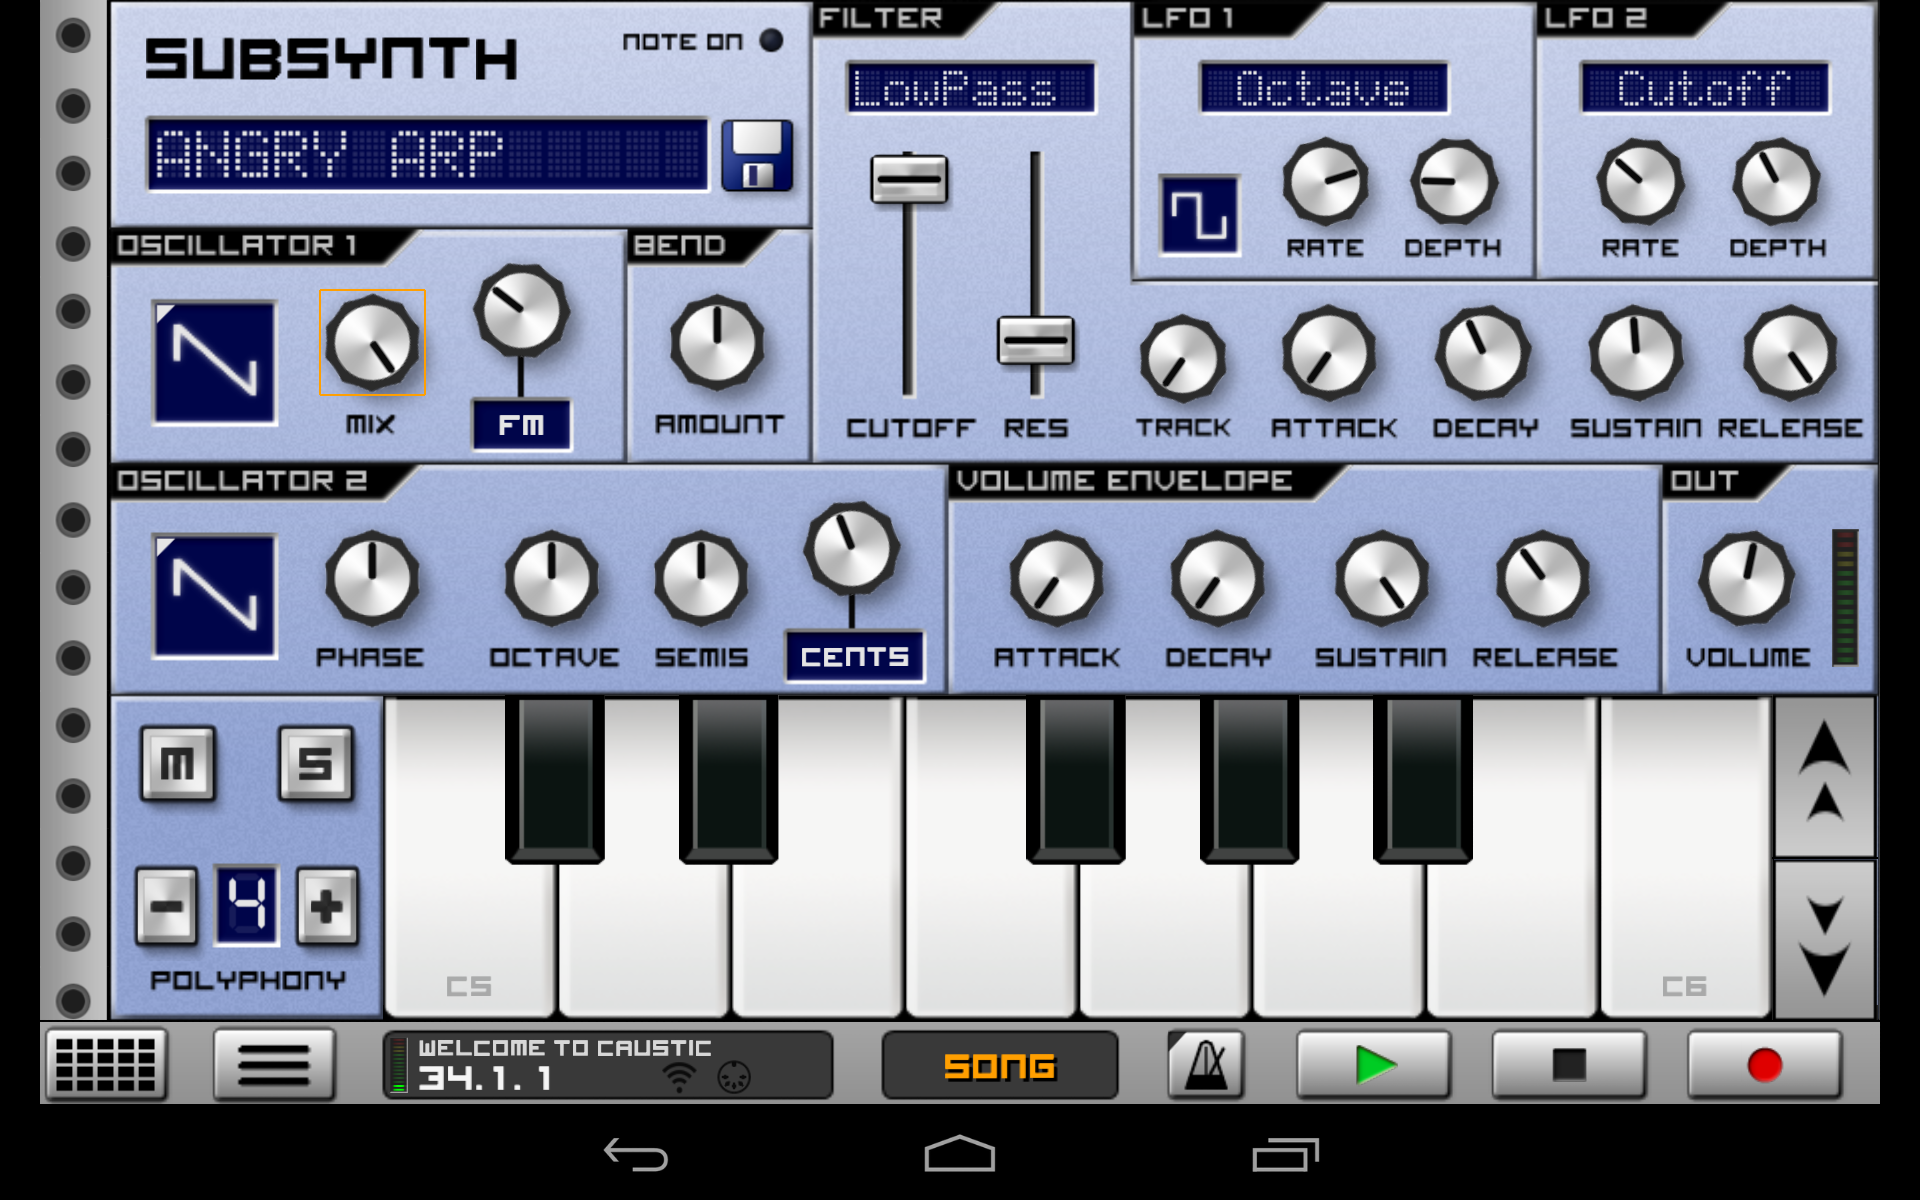
\includegraphics[width=0.6\textwidth]{caustic.png}
\caption{A screenshot of a subtractive synthesizer in Caustic}
\label{fig:caustic}
\end{figure}


\section*{Additional Hardware}

We do not expect to purchase additional hardware for this project. However, we
will be targeting different hardware for our final project. Michael Nye owns
a 2013 Nexus 7 that we believe will have better latency than the Motorola 
XOOM tablet, and we will be actively supporting this device for our project as 
well.


\section*{Existing tools}

Michael Nye has been working on ClickTrack\cite{clicktrack}, a C++ music
production tool, as a personal project.  In its present state, it contains
generic code for synthesis and filter design, as well as event handling code for
basic MIDI instruments. It contains only a very small number of actual filters.
We hope to expand this library and port it to Android for faster native signal
processing code. Alternatives for music production include Stanford University
Synthesis Toolkit\cite{stk}.

\begin{figure}[h]
\centering
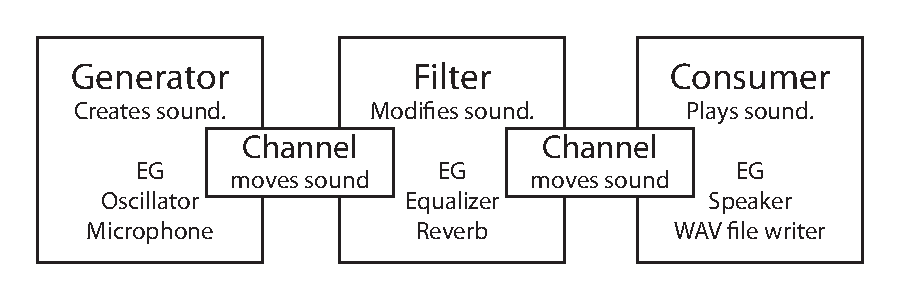
\includegraphics{clicktrack.pdf}
\caption{Basic ClickTrack architecture}
\label{fig:clicktrackarch}
\end{figure}


For the user interface, we intend to use Android's native graphics support.
Third party libraries will be considered if it becomes apparent that Android
alone cannot meet our interface needs.

The developer of popular Android synthesizer Caustic has expressed that his
measurements place touch to audio latency of some devices between 50ms and
100ms\cite{causticlatency}, which we feel is fast enough for potentially
satisfying interaction.  The open source audio accelerator
OpenSLES\cite{opensles} makes this possible, so we plan on integrating that into
our app pipeline.


\section*{Initial investigation}

Real time music synthesis is a task which requires very tight performance
characteristics. Due to this, designing a solid synthesis kit is highly
dependent on the OS and hardware platform it is deployed on. Unfortunately,
due to its highly portable nature, it is difficult to find hard numbers on
Android's performance. Due to this, our initial task will be to collect data
to characterize some aspects of Android performance metrics.

This will include numbers such as audio buffer latency, end-to-end latency from
screen press to sound out, and the overhead of calling native code functions.
This data will help influence the design of our interface and the underlying
structure of our system.

Accurately detecting audio latency will be difficult to do entirely inside the
Android ecosystem. One proposed experiment is as follows: Placing a microphone
next to the Android device and pressing an app-defined button that triggers
sound generation loudly enough for the microphone to hear the press. Record both
the manual press and the generated sound, then examine the resulting audio file
and compare the onset of each noise. On the device, we can also log the system
time of the touch event being registered and the audio being written out. This
should allow us to determing the latency between several different points on the
audio production path for Android code, native code, and any libraries that we
choose to use. The results should help us establish a baseline for latency and
indicate whether or not live performance, such as simulating presses of a piano
keyboard, is worth considering for the application.


\section*{Design tasks}

After investigations, the first task for our project is to port the ClickTrack
interface to Android.  ClickTrack is a C++ toolkit, and it contains no
dependencies other than those used to talk to the sound card and receive MIDI.
Thus, this task will focus on writing new end wrappers to give us access to
sound on Android. It will also require a new event handler to replace MIDI. If
all goes well, the majority of the code can be synchronized upstream with the
master ClickTrack repository.

Concurrently to porting ClickTrack, we will have to design interface code for
playing music. This interface will be based on scheduling music a few measures
at a time, and triggering loops. This interface code will then need to connect
to a scheduler that will allow it to communicate with the sound processing
backend to play sound. If latency permits it, a live performance option
simulating a keyboard might be considered.

\begin{figure}[h]
\centering
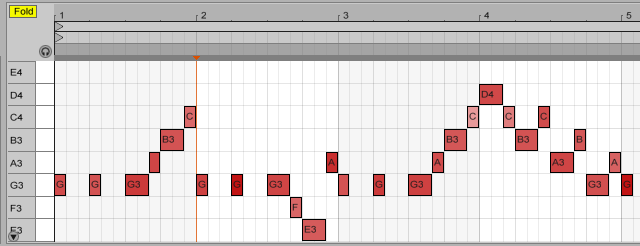
\includegraphics[width=0.9\textwidth]{abletonsequencer.png}
\caption{An example sequencer interface from Ableton Live, limited to a scale}
\label{fig:abletonsequencer}
\end{figure}

Once these two tasks are completed, we will have the building blocks of a live
performance system. The third step will then be to expand the breadth of our
filters. MATLAB can make prototyping of filters and synthesis techniques simple,
and the ClickTrack framework for desktop computers makes it easier to test C++
implementations of these. Ideally, we will thus be able to implement several
interesting effects into our app, to expand the performance possibilities.


\begin{thebibliography}{9}
    \singlespacing
    \bibitem{caustic}
    \url{https://play.google.com/store/apps/details?id=com.singlecellsoftware.caustic}

    \bibitem{clicktrack}
    \url{https://github.com/thenyeguy/ClickTrack}

    \bibitem{stk}
    \url{https://ccrma.stanford.edu/software/stk/}

    \bibitem{causticlatency}
    \url{http://www.reddit.com/r/Android/comments/1j6erw/android_43_latency_measurements/}

    \bibitem{opensles}
    \url{http://www.khronos.org/opensles/}

\end{thebibliography}


\section*{Proposed Schedule}

\begin{tabular}{| c || l |}
  \hline 
  Week 1 (Feb 16 - Feb 22) & Initial proposal and presentation Feb 18 \\ 
                           & Experiment with Android audio latency Feb 22 \\ \hline
  Week 2 (Feb 23 - Mar 2)  & Nye - Begin porting ClickTrack to Android \\
                           & Ryan -  Develop barebones sequencer, piano roll, or keyboard \\ &interface on Android \\ \hline
  Week 3 (Mar 9 - Mar 15)  & Spring break!  \\ \hline
  Week 4 (Mar 16 - Mar 22) & Nye - ClickTrack functionality on Android \\ 
                           & Ryan - Combine interface with ported audio production \\ \hline
  Week 5 (Mar 23 - Mar 29) & Nye - Finish port of ClickTrack with Java interface \\
                           & Ryan - Refactor and make robust interface \\ \hline
  Week 6 (Mar 30 - Apr 5)  & \textbf{Updates} \\
                           & Begin expanding functionality for additional instruments \\ & and effects\\ \hline
  Week 7 (Apr 6 - Apr 12)  &  Continue expanding functionality \\ \hline
  Week 8 (Apr 13 - Apr 19) & Continue expanding functionality. \\
                           & Spectrum and envelope visualization tools \\ \hline
  Week 9 (Apr 20 - Apr 26) & Nye - Additional effects and cleanup of audio engine \\
                           & Ryan - Additional effects and cleanup of interface \\ \hline
  Week 10 (Apr 27 - May 3) & Completed project and working demo  \\ \hline
  Week 11 (May 4 - May 11) & Final report  \\ \hline
\end{tabular}


\end{document}
